\documentclass[tikz, margin=3mm]{standalone}
\usetikzlibrary{chains,
                positioning}

\begin{document}
    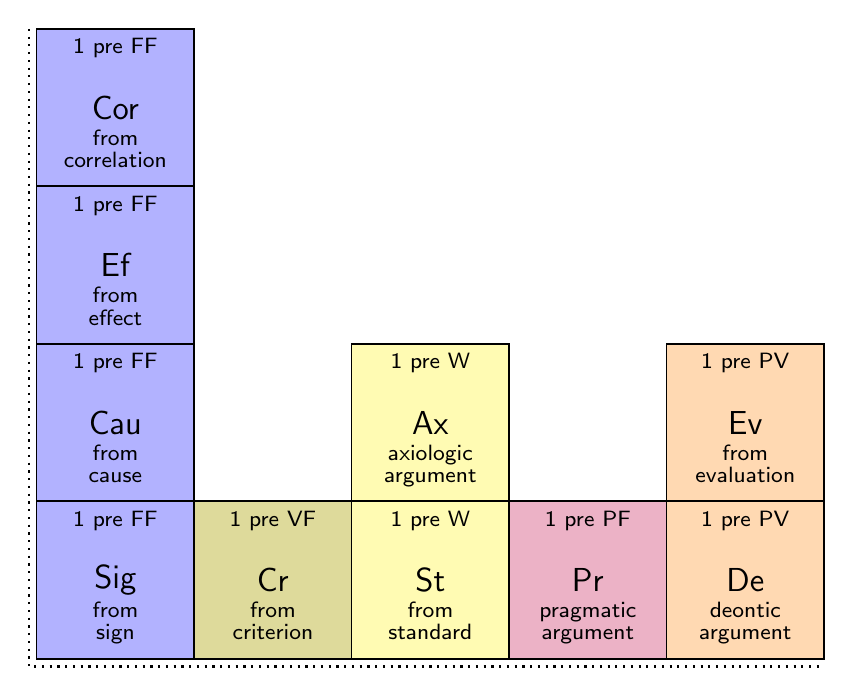
\begin{tikzpicture}[
node distance = 0pt,
  start chain = going above,
square/.style args = {#1/#2/#3}{%
        rectangle, draw, semithick,
        fill=#1,
        minimum size=20mm, inner sep=2mm, outer sep=0mm,
        font=\large\sffamily, 
        label={[anchor=north]above:#2},
        label={[anchor=south,yshift=0.5ex]below:#3},
        on chain},
every label/.append style = {%
        label distance=0pt, text depth=0.25ex, align=center,
        font=\footnotesize\sffamily\linespread{0.84}\selectfont}
                        ]
% 1. column, from bottom to top
\node (Sig) [square=blue!30/1 pre FF/from\\ sign]     {Sig};
\node (Cau) [square=blue!30/1 pre FF/from\\ cause]    {Cau};
\node (Ef)  [square=blue!30/1 pre FF/from\\ effect]   {Ef};
\node (Cor) [square=blue!30/1 pre FF/from\\ 
                                     correlation]   {Cor};
% 2. column, from bottom to top
\node (Cr)  [square=olive!30/1 pre VF/from\\ criterion,
             right=of Sig]                          {Cr};
% 3. column, from bottom to top
\node (St)  [square=yellow!30/1 pre W/from\\ standard,
             right=of Cr]                           {St};
\node (Ax)  [square=yellow!30/1 pre W/axiologic\\ 
                                      argument]     {Ax};
% 4. column, from bottom to top
\node (Pr)  [square=purple!30/1 pre PF/pragmatic\\ argument,
             right=of St]                           {Pr};
% 5. column, from bottom to top
\node (De)  [square=orange!30/1 pre PV/deontic\\ argument,
             right=of Pr]                           {De};
\node (Ev)  [square=orange!30/1 pre PV/from\\ 
                                       evaluation]  {Ev};
% Axes
\draw [dotted,thick] ([xshift=-1mm] Cor.north west) |- ([yshift=-1mm] De.south east);
\end{tikzpicture}
\end{document}
